\chapter{実験結果と考察}

\section{4種類のネットワークの精度}

\subsection{CNN}
浮動少数の重みを用いた一般的なCNNを用いた際のAccuracyとLossを図\ref{fig_cnn_acc},図\ref{fig_cnn_loss}に示す.
\begin{figure}[]
    \begin{center}
      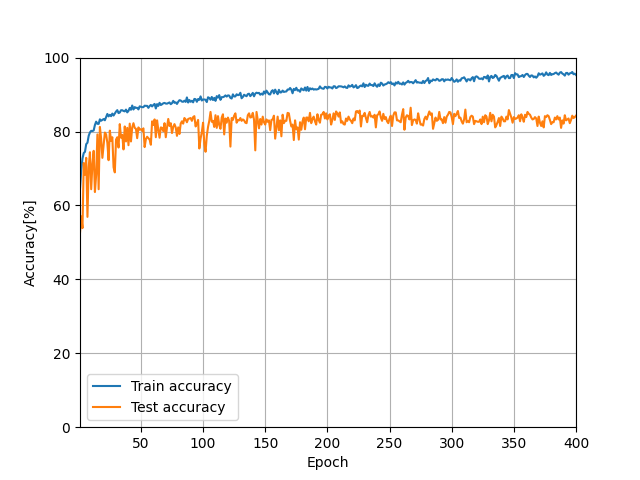
\includegraphics[scale = 0.5]{./chapter4/acc_cnn.png}
      \caption{CNNによるAccuracy}
      \label{fig_cnn_acc}
    \end{center}
\end{figure}
\begin{figure}[]
    \begin{center}
      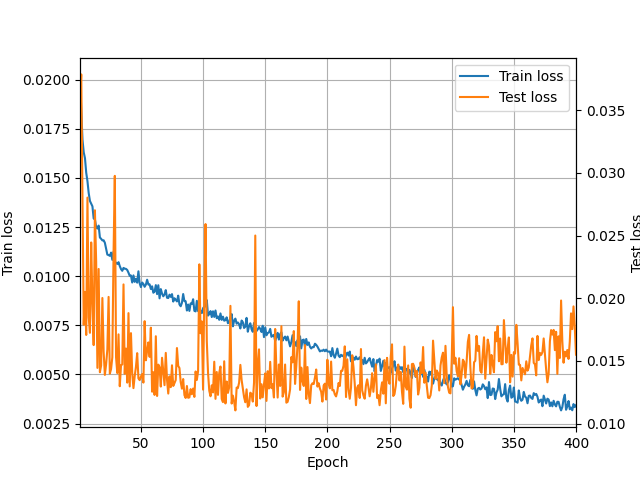
\includegraphics[scale = 0.5]{./chapter4/loss_cnn.png}
      \caption{CNNによるLoss}
      \label{fig_cnn_loss}
    \end{center}
\end{figure}

\subsection{BinaryConnect}
重みのみ2値化しBiasは通常のものを用いたネットワークを用いた際のAccuracyとLossを図に示す.

\subsection{Biasを含むBinaryConnect}
重み,Bias両方を2値化したネットワークを用いた際のAccuracyとLossを図に示す.